%%%%%%%%%%%%%%%%%%%%%%%%%%%%%%%%%%%%%%%%%%%%%%%%%%%%%%%%%%%%
\newcommand{\coursename}{Математический анализ 1 к. 2 с.}
\newcommand{\compiledby}{Даниил Гагарин$\frownie$в, gagarinovdaniil@gmail.com } % укажите свое имя
\newcommand{\coursedate}{Весна 2018 г.}
%%%%%%%%%%%%%%%%%%%%%%%%%%%%%%%%%%%%%%%%%%%%%%%%%%%%%%%%%%%%%%%%%%%%%%%%%%%%%%%%
% Преамбула для набора конспектов
% Версия 1.1
% Алексей Трошин. mailto: ai-troshin@yandex.ru

\documentclass[a4paper]{article}           % тип документа

\usepackage{geometry}     
              % задание полей текста
\geometry{left=30mm,right=10mm,top=20mm,bottom=20mm}
\usepackage[usenames]{color}
\usepackage{colortbl}
\usepackage{tikz}  
\usepackage{amsmath,amsfonts,amssymb}      % расширенная математика
\usepackage{xifthen}                       % удобный формат условий
\usepackage{graphicx}                      % поддержка рисунков
\usepackage{wrapfig}                       % поддержка обтекаемых рисунков
\usepackage{subcaption}                    % поддержка 'субрисунков'
\usepackage[makeroom]{cancel}              % поддержка зачеркиваний (сокращений)
\usepackage{ wasysym }
\usepackage{caption}                       % переопределение формата подписей
\captionsetup[figure]{labelsep=period}     % 'Рис. 1. ' вместо 'Рис. 1: '

\usepackage{unicode-math}                  % поддержка шрифта STIX Two
\defaultfontfeatures{Ligatures=TeX,Mapping=tex-text}
\setmainfont{STIX Two Text}
\setmathfont{STIX Two Math}

\usepackage{polyglossia}                   % поддержка языков в XeTeX
\setdefaultlanguage[spelling=modern]{russian}
\setotherlanguage{english}
\PolyglossiaSetup{russian}{indentfirst=true}

\sloppy                                    % строго соблюдать границы текста
\linespread{1.3}                           % коэффициент межстрочного интервала
\setlength{\parskip}{0.5em}                % вертик. интервал между абзацами

\setcounter{secnumdepth}{0}                % отключение нумерации разделов
\binoppenalty=1000                         % уменьшение переносов в формулах

\newcommand{\Def}{\textbf{Def.} }          % объявление новых макрокоманд

\newcommand{\Th}[1]{\textbf{Th\ifthenelse{\isempty{#1}}{}{ (#1)}.}}
\newcommand{\Consequence}[1]
           {\textbf{Следствие\ifthenelse{\isempty{#1}}{}{ #1}.}}
\newcommand{\Problem}[1]{\textbf{Задача\ifthenelse{\isempty{#1}}{}{ (#1)}.}}

\newcommand{\Remind}{\textbf{Напоминание.} }
\newcommand{\Note}{\textbf{Замечание.} }
\newcommand{\Statement}{\textbf{Утверждение.} }
\newcommand{\Proof}{\textbf{Доказательство:} }
\newcommand{\Prooff}{\textbf{Доказать:} }
\newcommand{\Solution}{\textbf{Решение.} }
\newcommand{\Endproof}{$\blacksquare$ }
\newcommand{\Endproofmath}{\ \blacksquare}
\newcommand{\Lemma}{\textbf{Лемма.} }
\newcommand{\Example}{\textbf{Пример} }
\newcommand{\Examples}{\textbf{Примеры.} }


\newcommand{\ds}{\displaystyle}
\newcommand{\opn}{\operatorname}

\newcommand{\va}{\mathbfit{a}}             % макрокоманды для векторов: a,b,c,n
\newcommand{\vb}{\mathbfit{b}}
\newcommand{\vc}{\mathbfit{c}}
\newcommand{\vn}{\mathbfit{n}}

\newcommand{\holds}{\hookrightarrow}       % символ 'выполняется'
\newcommand{\N}{\mathbb{N}}                % символ множества N
\newcommand{\Z}{\mathbb{Z}}                % символ множества Z
\newcommand{\Q}{\mathbb{Q}}                % символ множества Q
\newcommand{\R}{\mathbb{R}}                % символ множества R
\newcommand{\U}{\text{U}}                  % символ окрестности
\newcommand{\Uo}{\text{Ů}}                 % символ проколотой окрестности
\newcommand{\lito}{\bar{\bar \textrm{o}}}  % символ 'o малое'
\newcommand{\bigo}{\textrm{O}}             % символ 'o большое'
\newcommand{\Ue}{\U_{\varepsilon}}
\newcommand{\Uoe}{\Uo_{\varepsilon}}

\newcommand{\eqdef}{\stackrel {\mathrm{def}}{=}}

\newcommand{\notimplies}{\ \nRightarrow\ } % символ 'не следует'

\newcommand{\eq}{\,=\,}
\newcommand{\todo}{\textbf {ВСТАВИТЬ ПРИМЕРЫ С РИСУНКАМИ!!!} }

\newcommand{\RNumb}[1]{\uppercase\expandafter{\romannumeral #1\relax}}

\renewcommand{\thefootnote}                % добавление ')' к номеру сноски
             {\arabic{footnote})}



\usepackage{titleps}                       % колонтитулы

\newpagestyle{main}{
  \setheadrule{.4pt}                       % линия отбивки верхнего колонтитула
  \sethead{\coursename}{}{\ifnum\thepage=1 % ЛУ, Ц, ПУ верхнего колонтитула
    \compiledby\else\sectiontitle\fi}
  \setfootrule{.4pt}                       % линия отбивки нижнего колонтитула
  \setfoot{\coursedate}{}{\thepage} }      % ЛУ, Ц, ПУ нижнего колонтитула

\pagestyle{main}

\newcommand{\Le}{\leqslant}                % русский стиль нестрогих неравенств
\newcommand{\Ge}{\geqslant}
%%%%%%%%%%%%%%%%%%%%%%%%%%%%%%%%%%%%%%%%%%%%%%%%%%%%%%%%%%%%%%%%%%%%%%%%%%%%%%%%

%%%%%%%%%%%%%%%%%%%%%%%%%%%%%%%%%%%%%%%%%%%%%%%%%%%%%%%%%%%%
\begin{document}

\section{Семинар №3}

\subsection{Пространство $\R ^n$}

\Def \parbox[t]{0.95\linewidth} { 
	Метрическое пространство $\R ^n$ ---  множество элементов (точек) $ x = \underbrace{ 		\left( x_1,\, x_2,\ldots, x_n \right)}_{\textcolor{red}{x_i - \text{координаты}}}$ с заданным  
	
	расстоянием между ними: 

	$$ \rho(x,y) = \sqrt{\sum \limits_{i=1}^{n}  \; \left( x_i - y_i \right)^2} \ \text{\textcolor{red}			{(евклидова метрика)}} $$

}

\underline{Свойства $\rho(x,y)$ :}

~~\parbox[t]{0.95\linewidth} {
	1)$\rho(x,y) \Ge 0$ ; \ $\rho(x,y)\!=\!0 \Leftrightarrow x = y$;

	2)$\rho(x,y)=\rho(y,x);$
 
	3)$\forall z \in \R^n \holds \rho(x,y) \Le \rho(x,z) + \rho(z,y)$;\ \textcolor{red}{$\left(  \text{неравенство } \bigtriangleup \right) $ }
}

\Note \parbox[t]{0.95\linewidth} {
	$\R$ можно рассматривать как метрическое пространство $\R^n$ при $n = 1$; 
	
	в нем $\rho(x,y) = \left| y-x \right|$.
}

\Def $\underset{\textcolor{red}{\R^n \text{ --- линейное пространство}}} {\text{В } \R^n \text{вводятся операции}} $ $x+y \eqdef \left(x_1+y_1, ...,x_n+y_n\right)$ и $\lambda x \eqdef \left( \lambda x_1, ..., \lambda x_n \right)$.

\Def (Шаровая) $\varepsilon$ --- окрестность  точки $x^{(0)}$ : $\Ue (x^{(0)}) = \left\{x \ | \ \rho(x,x^{(0)})< \varepsilon \right\} $. 

\begin{figure}[h]
	\begin{center}
	    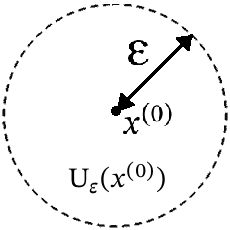
\includegraphics[width=0.15\textwidth]{1.png}
	  \end{center}
	\caption{\ $\varepsilon$ --- окрестность точки $x^{(0)}$}
\end{figure}

\Note Аналогично можно ввести прямоугольную, квадратную и другие окрестности.

\Def $\Uoe(x^{(0)})= \Ue (x^{(0)}) \setminus \left\{ x^{(0)} \right\} $

\Def Последовательность $\left\{ x^{(m)} \right\} $ --- отбражение $\N  \rightarrow \R^n$ $\textcolor{red}{\left( \forall m \in \N \ \text{поставлена в соответсвие точка} \ x^{(m)} \in \R^n \right)}$

\Def $\lim\limits_{m \to \infty} x^{(m)} = x^{(0)}$, если 
$$\forall \varepsilon > 0 \ \exists N \in \N : \forall m \Ge N \holds \textcolor{red}{\underbrace {\textcolor{black}{\rho (x^{(m)}, x^{(0)})< \varepsilon}}_{\text{\normalsize $\left( x^{(m)} \in \Uoe(x^{(0)}) \right)$}}} $$

\Note $\lim\limits_{m \to \infty} x^{(m)} = x^{(0)} \Leftrightarrow \lim\limits_{m \to \infty} \underbrace{ \rho (x^{(m)}, x^{(0)})}_{\textcolor{red}{\substack {\text{числовая} \\ \text{последовательность}}}}= \ 0 \Leftrightarrow \underbrace{\lim\limits_{m \to \infty} x_i^{(m)} = x_i^{(0)}  }_{\textcolor{red}{\substack {\text{пределы n числовых} \\ \text{последовательностей}}}} , \ i = 1, \ldots, n$.

\Def $\lim\limits_{m \to \infty} x^{(m)} = \infty , \text{если } \rho (x^{(m)}, 0) = \infty $.

\Problem{} Д-ть: $\lim\limits_{m \to \infty} \rho(x^{(m)}, 0) = \infty \Leftrightarrow \forall a \in \R^n \holds 
\lim\limits_{m \to \infty} \rho(x^{(m)}, a) = \infty$

\Proof  

~~ \parbox[t]{0.95\linewidth} {
	\textbf{"$\Rightarrow$"} \parbox[t]{0.95\linewidth} {
		пусть $\lim\limits_{m \to \infty} \rho(x^{(m)}, 0) = \infty \Rightarrow \forall a \in \R^n 	\holds 			\rho(x^{(m)}, a) + \rho(a, 0) \overset {\textcolor{red}{\text{н-во } \bigtriangleup }} {\Ge} 				\rho(x^{(m)}, 0) \Rightarrow$

		$\Rightarrow \rho(x^{(m)}, a) \Ge \underbrace{\rho(x^{(m)}, 0)}_{\substack{\ \qquad 					\downarrow \ m \to \infty  \\ \infty}} - \underbrace{\rho(a,0)}_{\substack{\textbardbl \\ const}} 		\Rightarrow \rho(x^{(m)}, a) \underset {m \to \infty} {\longrightarrow} \infty $;
	}
}

%%%%%%%%%%%%%%%%%%%%%%%%%%%%%%%%%%%%%%%%%%%%%%%%%%%%%%%%%%%%%%
\newpage 

~~ \parbox[t]{0.95\linewidth} {
	\textbf{"$\Leftarrow$"} пусть $\forall a \in \R^n \holds \lim\limits_{m \to \infty} \rho(x^{(m)}, a) = 		\infty$. Возьмем $a = 0 \in \R^n \Rightarrow  \lim\limits_{m \to \infty} \rho(x^{(m)}, 0) = \infty$. 			\Endproof
}

\Def $\left\{ x^{(m)} \right\}$ называется ограниченной, если $\underline{\text{числовая}}$ последовательность $\left\{ \rho(x^{(m)}, 0)  \right\}$ ограничена.

\Th{Больцано-Вейерштрасса}

~~ \parbox[t]{0.95\linewidth} {
	Из $\forall$ ограниченной последовательности можно выделить сходящуюся 					подпоследовательность.
}

\Th{Критерий Коши сходимости последовательности} 

~~\parbox[t]{0.95\linewidth} {
	$\left\{ x^{(m)} \right\}$ сходится $\Leftrightarrow \forall \varepsilon \!>\! 0 \ 
	\exists N \! \in \! \N \! : $ 
	$\forall m \Ge N, \forall p \in \N \holds \rho (x^{(m)}, x^{(m+p)}) < \varepsilon$.
}

\smallskip

\subsection {Классификация множеств в $\R^n$}

\fbox{\textbf{\RNumb{1}}} \textbf{Открытые множества.}

\Def х называется внутренней точкой м-ва $E \subset\R^n$, если $\exists \Ue(x) \subset E$.

\Def Внутренность мн-ва $E \subset\R^n$ : $intE = \left\{ x \, | \, x \text{--- внутренняя т. } E \, \right\}$.

\Example $int[1;2]=(1;2)$ \textcolor{red}{(внутренность отрезка --- интервал)}

\Def Мн-во $E \subset \R^n$ называется открытым, если $\forall x \in E$ является внутренней т. E, т.е. \textcolor{red}{\fbox{\textcolor{black}{$intE = E$}}}

\Note  $\varnothing, \R^n$ --- открытые множества. \textcolor{red}{\fbox{!}}

\Examples \parbox[t]{0.95\linewidth} {
	$n = 1$: \parbox[t]{0.95\linewidth} {
		$(a,b)$ --- открытое мн-во 
		\begin{picture}(1,1)
			\put(0,0){\line(1,0){80}}
			\put(12.5,-10){a}
			\put(15,0){\circle{5}}
			\put(62.5,-10){b}
			\put(65,0){\circle{5}}
			\put(37.5,-10){x}
			\put(40,0){\circle*{5}}
			\put(47.5,-3){)}
			\put(27.5,-3){(}
			\put(17.5,10){\textcolor{red}{$\exists \ \varepsilon$ окр-ть}}
		\end{picture}

		\bigskip \bigskip
		
		$[a,b]$ --- не открытое мн-во 
		\begin{picture}(1,1)
			\put(0,0){\line(1,0){80}}
			\put(12.5,-10){a}
			\put(15,0){\circle*{5}}
			\put(62.5,-10){b}
			\put(65,0){\circle*{5}}
			\put(72.5,-3){)}
			\put(52.5,-3){(}
			\put(42.5,10){\textcolor{red}{$\nexists \ \varepsilon$ окр-ть}}
			\put(85,-2.5) {\textcolor{black}{(a,b не являются внутренними точками)}}
		\end{picture}
		
	}
	
	\bigskip \bigskip 

	$n = 2$: \parbox[t]{0.95\linewidth} {
		
	}


}

\begin{figure}[h]
	\begin{center}
	    	\begin{minipage}[h]{0.49\linewidth}
  			\center {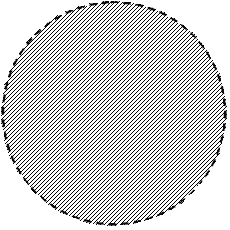
\includegraphics[width=0.5\linewidth]{2.png} }
		\end{minipage}
		\hfill
		\begin{minipage}[h]{0.49\linewidth}
  			\center {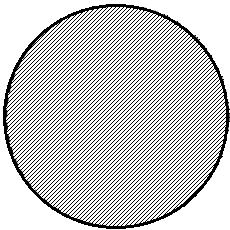
\includegraphics[width=0.5\linewidth]{3.png} }

		\end{minipage}
		\begin{minipage}[h]{1\linewidth}
			\begin{tabular}{p{0.49\linewidth}p{0.49\linewidth}}
				\centering {$\left\{ (x,y) | x^2 + y^2 < 1 \right\}$ --- открытое} & 
				\centering {$\left\{ (x,y) | x^2 + y^2 \Le 1 \right\}$ --- не открытое} \\
			\end{tabular}
		\end{minipage}
	\end{center}
	\vspace*{-1cm}
	\caption {}
\end{figure}

\Th{} A, B --- открытые мн-ва $\Rightarrow \underbrace{A \cup B}_{\text{а)}}$ открытое и $\underbrace{A \cap B}_{\text{б)}}$ открытое.

\Proof (см. Рис. 3)

~~ \parbox[t]{0.95\linewidth}{
	\textbf{а)} 
	\parbox[t]{0.95\linewidth}{
		пусть $x \in A \cup B \Rightarrow x \in a \text{ или } x \in B$. Если $x \in A$, то \ $					\exists \Ue(x) \subset A \subset A \cup B \Rightarrow $

		$ \Rightarrow x \text {--- внутренняя точка } A \cup B$. Аналогично при $x \in B$.
	}

	\textbf{б)} 
	\parbox[t]{0.95\linewidth}{
		если $A \cap B = \varnothing$ очев. Пусть $A \cap B \neq \varnothing$. Пусть $x \in 				A \cap B \rightarrow x \in A$ и $x\in B$.  \\ x --- внутр. для A $\Rightarrow \exists 					\U_{\varepsilon_A}(x) \subset A$; 

		x --- внутр. для B $\Rightarrow \exists \U_{\varepsilon_B}	(x) \subset B$. 
		
		Возьмем 	$ \varepsilon = min \left\{ \varepsilon_A, \varepsilon_B \right\}$.  Тогда $\Ue(x) 			\subset A \cap B \Rightarrow x$ --- внутренняя для $A \cap B$. \Endproof
	}
	
}

%%%%%%%%%%%%%%%%%%%%%%%%%%%%%%%%%%%%%%%%%%%%%%%%%%%%%%%%%%%%%%
\newpage 

\begin{figure}[h]
	\begin{center}
	    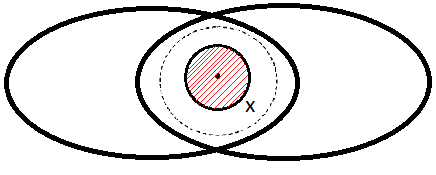
\includegraphics[width=0.4\textwidth]{4.png}
	  \end{center}
	\caption{Иллюстрация к доказательству \textbf{Th.} }
\end{figure}

\Consequence{} \parbox[t]{0.95\linewidth}{$\cup \ \underline{\text{любого}}$ числа открытых множеств --- открытое множество.

$\cap \ \underline{\text{конечного}}$ числа открытых множеств --- открытое множество$^{ \textbf{*}}$}

\Note Для бесконечного числа открытых множеств \textbf{*} выполняется не всегда.

\Def $\forall$ открытое мн-во, содержащее т.x, называется окрестностью т.x и обозн. $\U(x)$. Аналогично $\Uo(x)$. \textcolor{red}{\fbox{!}}

\smallskip

\fbox{\textbf{\RNumb{2}}} \textbf{Замкнутые множества.}

\Def $x \in \R^n$ --- т. прикосновения мн-ва $E \subset \R^n$, если $\forall \U(x) \cap E \neq \varnothing$.

\Def Замыкание множества $E \subset \R^n$ : $\overline{E} = \left\{ x \, | \, x \text{ --- т. прикосновения E}\right\}$

\Examples \parbox[t]{0.95\linewidth} {
	$n = 1$: \parbox[t]{0.95\linewidth} {
		\begin{picture}(0,0)
			\put(5,0){\line(1,0){60}}
			\put(2.5,-10){a}
			\put(5,0){\circle*{5}}
			\put(62.5,-10){b}
			\put(65,0){\circle*{5}}
			\put(70,-2.5) {\textcolor{black}{замкнутое, не открытое}}
		\end{picture}

		\bigskip \bigskip
		
		\begin{picture}(0,0)
			\put(5,0){\line(1,0){57.5}}
			\put(2.5,-10){a}
			\put(5,0){\circle*{5}}
			\put(62.5,-10){b}
			\put(65,0){\circle{5}}
			\put(70,-2.5) {\textcolor{black}{не замкнутое, не открытое}}
		\end{picture}

		\bigskip \bigskip
		
		\begin{picture}(0,0)
			\put(7.5,0){\line(1,0){55}}
			\put(2.5,-10){a}
			\put(5,0){\circle{5}}
			\put(62.5,-10){b}
			\put(65,0){\circle{5}}
			\put(70,-2.5) {\textcolor{black}{не замкнутое, открытое}}
		\end{picture}
		
	}
	
	\bigskip \bigskip 

	$n = 2$ (см. Рис. 4): \parbox[t]{0.95\linewidth} {
		E = открытый круг $\cup$ отдельная точка;

		$\overline{E}$ = круг, включая границу $\cup$ отдельная точка.
	}
}

\begin{figure}[h]
	\begin{center}
	    	\begin{minipage}[h]{0.49\linewidth}
  			\center {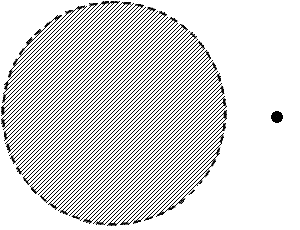
\includegraphics[width=0.5\linewidth]{6.png} }
		\end{minipage}
		\hfill
		\begin{minipage}[h]{0.49\linewidth}
  			\center {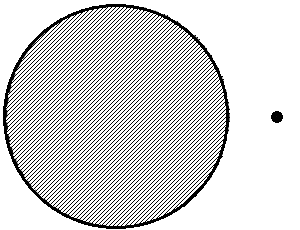
\includegraphics[width=0.5\linewidth]{5.png} }

		\end{minipage}
		\begin{minipage}[h]{1\linewidth}
			\begin{tabular}{p{0.49\linewidth}p{0.49\linewidth}}
				\centering {E} & 
				\centering {$\overline{E}$} \\
			\end{tabular}
		\end{minipage}
	\end{center}
	\vspace*{-1cm}
	\caption {}
\end{figure}

\Note $\varnothing$, $\R^n$ --- замкнутые множества \textcolor{red}{(и одновременно открытые)        
 \fbox{!}}

\Def $\R^n \backslash E$ называется дополнением множества E.

\Th{} E открыто $\Leftrightarrow \R^n \backslash E$ замкнуто. \textcolor{black}{$\left( \text{E замкнуто $\Leftrightarrow \R^n \backslash E$ открыто} \right)$}

\Th{законы де Моргана} 

~~\parbox[t]{0.95\linewidth}{
	$\R^n \backslash \big( \bigcup\limits_i E_i \big) = \bigcap\limits_i \big( R^n \backslash E_i \big)$

	$\R^n \backslash \big( \bigcap\limits_i E_i \big) = \bigcup\limits_i \big( R^n \backslash E_i \big)$
}

\Consequence{} A,B --- замкнутые множества $\Rightarrow A \cap B$ замкнуто и $A \cup B$ замкнуто.

\Consequence{} 
\parbox[t]{0.95\linewidth}{
	$\cap \ \underline{\text{любого}}$ числа замкнутых множеств --- замкнутое множество.

	$\cup \ \underline{\text{конечного}}$ числа замкнутых множеств --- замкнутое множество$^{ 	\textbf{*}}$
}

%%%%%%%%%%%%%%%%%%%%%%%%%%%%%%%%%%%%%%%%%%%%%%%%%%%%%%%%%%%%%%
\newpage

\Note Для бесконечного числа замкнутых множеств \textbf{*} выполняется не всегда.

\Example  $\bigcup\limits_{n=1}^{\infty} \underbrace{\left[ -1 + \frac{1}{n}, 1 - \frac{1}{n} \right]}_{\text{зам.}} = \underbrace{(-1, 1)}_{\text{не зам.}}$

\smallskip

\fbox{\textbf{\RNumb{3}}} \textbf{Изолированные и предельные точки.}

\Def $x \in E$  --- изолированная точка множества $E \subset \R^n$, если $\exists \Uoe(x) : \Uoe(x) \cap E = \varnothing$.

\Example 
\begin{figure}[h]
	\begin{center}
	    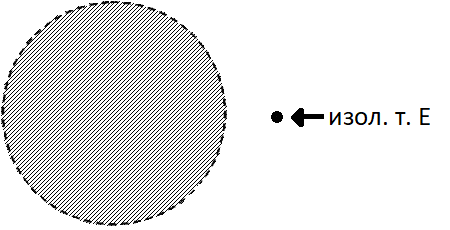
\includegraphics[width=0.4\textwidth]{9.png}
	  \end{center}
	\caption{}
\end{figure}

\Def x --- предельная точка множества $E \subset \R^n$, если $\forall \, \Uo(x) \cap E \neq \varnothing$

\Note x --- предельная точка E $\Leftrightarrow \exists$ последовательность Гейне ${x^{(m)}} \subset E$, сходящаяся к x.

\Note \parbox[t]{0.95\linewidth}{
	$\forall$ мн-ва $E \subset \R^n \holds$ \{т-ки прикосновения\} = \{предельные т-ки\}  
	$\cup$ \{изолированные т-ки\},

	причем \{предельные т-ки\}  $\cap$ \{изолированные т-ки\} $= \varnothing$.
}

\smallskip

\fbox{\textbf{\RNumb{4}}} \textbf{Границы множеств.}

\Def x --- граничная точка множества $E \subset \R^n$, если $\forall \U(x)$ содержит как точки из E, так и из $\R^n \backslash E$.

\Def Граница множества  $E \subset \R^n$ : $\partial E = \left\{ x  \text{ | x --- граничная точка } E \right\}$.

\Example граница круга и изолированной точки

\begin{figure}[h]
	\begin{center}
	    	\begin{minipage}[h]{0.49\linewidth}
  			\center {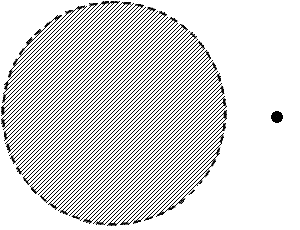
\includegraphics[width=0.5\linewidth]{6.png} }
		\end{minipage}
		\hfill
		\begin{minipage}[h]{0.49\linewidth}
  			\center {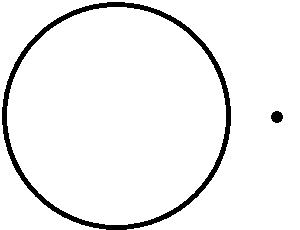
\includegraphics[width=0.5\linewidth]{7.png} }
		\end{minipage}
		\begin{minipage}[h]{1\linewidth}
			\begin{tabular}{p{0.49\linewidth}p{0.49\linewidth}}
				\centering {E} & 
				\centering {$\partial E$} \\
			\end{tabular}
		\end{minipage}
	\end{center}
	\vspace*{-1cm}
	\caption {}
\end{figure}

\Examples E-? : \parbox[t]{0.95\textwidth}{
1)$\partial E \subset$ и $\partial E \neq E$ --- замкнутый круг

2)$\partial E = E$ --- окружность, точка

3)$\partial E \cap E = \varnothing$  --- открытый круг

4)$\partial E = \varnothing$  --- $\R^n$

5)$\partial E \supset E$ и $\partial E \neq E$ --- $\Q$; \ \tikz{\draw (-1,-1) -- (-0.81,-0.81); \path[draw=red] (-0.75,-0.75) circle (1mm); \draw (-0.69,-0.69) -- (-0.5,-0.5);} .}

%%%%%%%%%%%%%%%%%%%%%%%%%%%%%%%%%%%%%%%%%%%%%%%%%%%%%%%%%%%%%%

\newpage

\smallskip

\fbox{\textbf{\RNumb{5}}} \textbf{Связность множества. Области и компакты.}

\Remind 

~~\parbox[t]{0.95\linewidth} {
	Непрерывная (параметрически заданная) кривая $	\Gamma \subset \R^n$ -- множество 		точек, заданное как непрерывное отображение отрезка $\alpha \Le t \Le \beta$: 
	$$ \Gamma = \left\{ x(t) = (x_1(t), \ldots, x_n(t)) | t \in [\alpha,\beta] \right\}$$
}

\Def \parbox[t]{0.95\linewidth} {
	Множество $E \subset \R^n$ называется \underline{линейно связным}, если $\forall$ его 2 			точки можно соединить непрерывной кривой $\Gamma \subset E$.
}

\Note Множество, состоящее из 1 точки, считается линейно связным.

\Example
\begin{figure}[h]
	\begin{center}
	    	\begin{minipage}[h]{0.49\linewidth}
  			\center {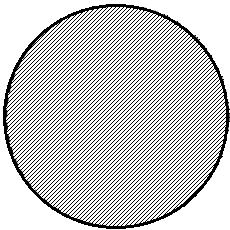
\includegraphics[width=0.5\linewidth]{3.png} }
		\end{minipage}
		\hfill
		\begin{minipage}[h]{0.49\linewidth}
  			\center {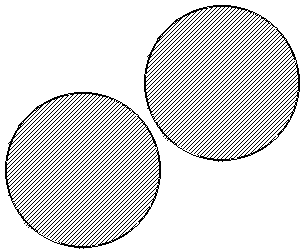
\includegraphics[width=0.5\linewidth]{8.png} }
		\end{minipage}
		\begin{minipage}[h]{1\linewidth}
			\begin{tabular}{p{0.49\linewidth}p{0.49\linewidth}}
				\centering {линейно связно} & 
				\centering {не линейно связно} \\
			\end{tabular}
		\end{minipage}
	\end{center}
	\vspace*{-1cm}
	\caption {}
\end{figure}

\Def Множество $E \subset \R^n$ называется областью, если оно открыто и линейно связно.

\Def Множество $E \subset \R^n : E \neq \varnothing $, называется компактом, если оно замкнуто и ограничено.

\Examples Интервал -- область, отрезок --- компакт.

\smallskip

\subsection{Дополнение к множествам в $\R^n$}

\fbox{\textbf{\RNumb{1}}} \ \parbox[t]{0.95\linewidth}{\Def Множество $E \subset \R^n$ называется \underline{связным}, если  $\forall$ его разбиения $E=\underset{\substack {\cancel{\textbardbl} \\ \varnothing}}{A} \cup \underset{\substack {\cancel{\textbardbl} \\ \varnothing}}{B}$, $A \cap B = \varnothing \holds A \cap \overline{B} \neq \varnothing$.

\Example \parbox[t]{0.95\linewidth}{
	связное, но не линейно связное множество : $E = \Big\{ (x,y) | x \Ge 0, y = \left\{ 					\substack{\sin{\frac{1}{x}}, x\ne0 \\ 0, x = 0} \right\}$.

	E --- график функции, имеющей точки разыва \RNumb{2} рода $\Rightarrow$ не линейно 			связное;

	но $\{(0,0)\} \cap \overline{E \backslash \{(0,0)\}} = \{(0,0)\} \ne \varnothing \Rightarrow$ E 			связно.
}

\smallskip

\Note E линейно связно $\Rightarrow$ E связно.}

\fbox{\textbf{\RNumb{2}}} \ \parbox[t]{0.95\linewidth}{ \Th{лемма Гейне-Бореля}  Пусть $K \subset \R^n$ --- компакт и $\left\{ G_k\right\}_{k=1}^\infty$ --- его $\overbrace {\text{покрытие}}^{K \subset \bigcup\limits_{k=1}^{\infty} G_k} $ \\ открытыми мн-ми. Тогда из $\left\{ G_k\right\}_{k=1}^\infty$  можно выделить \underline{конечное} подпокрытие $\left\{ G_k\right\}_{k=1}^m$ компакта K.

\Proof для $\R$  и случая $K = \left[a,b\right]$

~~\parbox[t]{0.95\linewidth}{Предположим обратное $\Rightarrow$ одну из половин $\left[a,\frac{a+b}{2} \right], 
\left[\frac{a+b}{2}, a \right]$ нельзя покрыть \\ конечным подпокрытием. Делим этот отрезок пополам и т.д. Получаем СВО с длиной $\rightarrow$ 0, \\ стягивающуюся к $x_0 \in [a,b]. \ x_0 \in$ одному из $G_k \Rightarrow$ начиная с некоторого шага деления отрезок целиком $\subset G_k$ ?! \Endproof}

\smallskip

\underline{Примеры использования:} \parbox[t]{0.95\linewidth}{
	
1) доказательство Th Кантора о РН $f(x)$ на [a,b]

2)задача: доказать, что $\bigcup\limits_{k=1}^{\infty} \U_{\frac{1}{2^k}} (q_k) \neq \R$ }
} 

%%%%%%%%%%%%%%%%%%%%%%%%%%%%%%%%%%%%%%%%%%%%%%%%%%%%%%%%%%%%%%

\newpage

\Problem{\&2 9.2} Является ли область определения $f(x,y) = \sqrt{x \sin{y}}$ замкнутым? открытым? областью?

~~\parbox[t]{0.95\linewidth}{

\Statement $\overline{E} = intE \cap \partial E$

~~\parbox[t]{0.95\linewidth} {\Proof  Пусть $x \in \overline{E} \Rightarrow \forall \U(x)$ содержит $x_1 \in E$. Либо $\exists \U^{(1)}(x)$, целиком $\subset E$, либо

 $\forall \U(x)$ содержит $x_2 \notin  E$. В первом случае $x \in intE$, во втором x $\in \partial E$ \Endproof
 
\Consequence{} $\partial E \subset E \Rightarrow \overline{E} = E. \left(  \overline{E} = \underbrace{intE}_{\substack {\cap \\ E}} \cup  \ \partial E  \right)$
}

\textbf{Решение:}

~~\parbox[t]{0.95\linewidth} {

Обозначим область определения $D$. $\partial D = \left\{ (0,y) \ | \ y \in \R \right\} \cup \left\{ (x,2\pi n) \ | \ x \in \R, n \in \Z \right\} \subset D \Rightarrow \overline{D} = D \Rightarrow $

$\Rightarrow$ \textbf{ D замкнуто.}

$\left\{ \substack {\text{ \normalsize $\partial D \subset D \Rightarrow $ \textbf{D не является открытым} $\Rightarrow$\textbf{D не область.}}   \\ \text{ \normalsize $\partial D \ne \varnothing$ }\hfill } \right. \ $ 

\smallskip

\Note \text{D линейно связно} 
}
}

\begin{figure}[h]
	\begin{center}
	    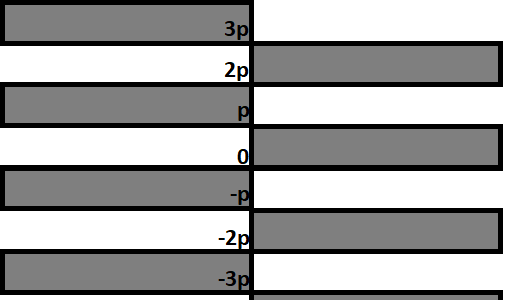
\includegraphics[width=0.4\textwidth]{10.png}
	  \end{center}
	\caption{Иллюстрация к задаче \&2 9.2}
\end{figure}

\Problem {\&1 13}  $f \in \mathbb{C} \; (\R), \ y_0 \in \R. \ \Prooff \ S = \left\{ x \; | \; f(x) > y_0 \right\}$ открыто.

~~\parbox[t]{0.95\linewidth} {
\textbf{План:} берем $x_0 \in S$, берем $\varepsilon = \frac {f(x_0)-y_0}{2}$, показываем, что $x_0 \in int S$.
}

\smallskip

\subsection{Функции многих переменных}

\Def $y = f(x) = f(x_1, \ldots, x_n)$ --- отображение $X \rightarrow \R$, где $X \subset \R^n$ --- множество  определения. 

Рассмотрим $f(x)$ на множестве $E \subset X$; пусть $x^{(0)}$ --- предельная точка $E$.

\parbox[t]{0.95\linewidth}{
	\Def (предел $f(x)$ в точке  $x^{(0)}$ по множеству $E$)
	
	$\lim\limits_{\substack {x \to x^{(0)} \\ x \; \in \; E}} f(x) = a$, если 
	$\left[ \substack { 
		\text{\normalsize по Гейне: $\forall \ \{ x^{(m)} \} \subset E \ \backslash \ $  
		 $\{ x^{(0)} \}: \  \lim\limits_{m \to \infty} x^{(m)} = x^{(0)} \holds$
		$ \lim\limits_{m \to \infty} f( x^{(m)}) = a $}
		\\
		\text{\normalsize по Коши: $\forall \varepsilon > 0 \ \exists \delta > 0 : \forall x \in 					\Uo_{\delta} (x^{(0)}) \cap E \holds | f(x) - a | < \varepsilon $}\hfill
	 } \right. $
}

\textbf{Обозначения:} $\lim\limits_{\substack {x \to x^{(0)} \\ x \; \in \; E }} f(x) = $
$\lim\limits_{\substack {\rho(x,x^{(0)}) \to 0 \\ x \; \in \; E}} f(x) =$
$\lim\limits_{\substack {x_1 \to x^{(0)}_1 \\ \vdots \\ x_n \to x^{(0)}_n \\ (x_1, \ldots, x_n) \in E} } f(x) $.

\Example функция Дирихле $D(x) =$ 
$\left\{ \substack { 
		\text{\normalsize $1, x \in \Q$}
		\\
		\text{\normalsize $0, x \in \mathbb{I}  $ \hfill}
 }\right. $ 
$\lim\limits_{\substack{ x \to 0 \\ x \in \Q}}D(x) = 1$, $\lim\limits_{\substack{ x \to 0 \\ x \in \mathbb{I}}}D(x) = 0$.

\parbox[t]{0.95\linewidth}{\Note в $\R^n$ сохраняются основные свойства пределов (\textbf{Th} об арифметический действиях, \\ свойства, связанные с неравенствами, понятия бесконечно малых и бесконечно больших функций).}

\Def (предел $f(x)$ в точке $x^{(0)}$)

~~Пусть $f(x)$ определена в некоторой $\Uo(x^{(0)})$. $$\lim\limits_{x \to x^{(0)}} f(x) \ \ \ \ \eqdef 
\lim\limits_{\substack {x \to x^{(0)} \\ x \; \in \; \Uo(x^{(0)}) }} f(x)$$.

%%%%%%%%%%%%%%%%%%%%%%%%%%%%%%%%%%%%%%%%%%%%%%%%%%%%%%%%%%%%%%

\newpage

\Th{} \parbox[t]{0.95\linewidth}{ Пусть $f(x)$ определена в некоторой $\Uo(x^{(0)}).  \lim\limits_{x \to x^{(0)}} f(x) = a \Leftrightarrow \forall E \subset X : $ \\
$x^{(0)}$ --- предельная точка $E \holds \lim\limits_{\substack {x \to x^{(0)} \\ x \; \in \; E }} f(x) = a$ }

\end{document}